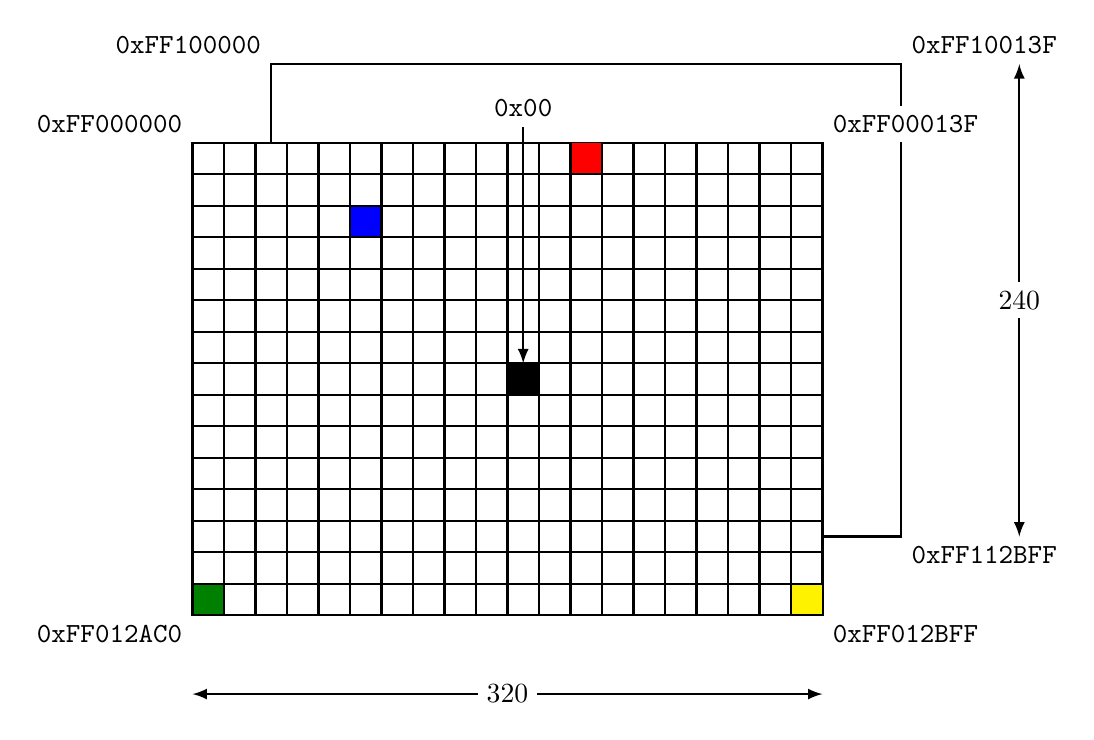
\begin{tikzpicture}[>=latex, thick]
    % frame 1
    \begin{scope}[shift={(1,1)}]
        \draw (0, 0) rectangle (8, 6);
        \draw
            node (FF100000) at (0, 6) {}
            node (FF10013F) at (8, 6) {}
            node (FF112BFF) at (8, 0) {}
            node (FF112AC0) at (0, 0) {}
        ;
        \draw 
            (FF100000.center) node [above left] {{\tt 0xFF100000}}
            (FF10013F.center) node [above right] {{\tt 0xFF10013F}}
            (FF112BFF.center) node [below right] {{\tt 0xFF112BFF}}
            %(FF112AC0.center) node [below left] {{\tt 0xFF112AC0}}
        ;
        \draw [<->] 
            (9.5, 6) --++ (0, -6) node [midway, fill=white] {240}
        ;
    \end{scope}

    % frame 0
    \draw [fill=white] (0, 0) rectangle (8, 6);
    \draw
        node (FF000000) at (0, 6) {}
        node (FF00013F) at (8, 6) {}
        node (FF012BFF) at (8, 0) {}
        node (FF012AC0) at (0, 0) {}
        
        (FF000000.center) node [above left] {{\tt 0xFF000000}}
        (FF00013F.center) node [above right, fill=white] {{\tt 0xFF00013F}}
        (FF012BFF.center) node [below right] {{\tt 0xFF012BFF}}
        (FF012AC0.center) node [below left] {{\tt 0xFF012AC0}}
    ;
    \draw [<->] 
        (0, -1) --++ (8, 0) node [midway, fill=white] {320}
    ;
    %% algumas cores
    \fill [green!50!black]  (0,0)       rectangle +(0.4, 0.4);
    \fill [red]    (4.8, 5.6)  rectangle +(0.4, 0.4);
    \fill [blue]   (2, 4.8)    rectangle +(0.4, 0.4);
    \fill [yellow] (7.6,0)     rectangle +(0.4, 0.4);
    \fill         (4, 2.8)    rectangle +(0.4, 0.4);
    
    \draw [<-] (4.2, 3.2) --++ (0, 3) node [above] {\tt 0x00};
    %% grade
    \foreach \i in {0, 0.4, 0.8, ..., 8} {
        \draw (\i, 0) --++ (0, 6);
    }
    \foreach \i in {0, 0.4, 0.8, ..., 6} {
        \draw (0, \i) --++ (8, 0);
    }
\end{tikzpicture}